\chapter{Experiments}\label{ch:experiments}
All experiments described in this chapter are executed in a test environment at Nikhef. The visualization of the test environment is displayed in figure \ref{fig:testenv}. \\ 

\begin{figure}[H]
  \includegraphics[scale=0.45]{images/testenv.pdf}
  \caption{Used environment for experiments.}
  \label{fig:testenv}
\end{figure}

The figure shows five server systems, of which three identical servers (A, B and C in table \ref{tab:testmachines}) are used to perform the tests whose results are described in this paper.
During the experiments 2 extra machines (D and E in table 4.1), both containing 100Gb/s Mellanox cards, have been introduced in the network. All servers were connected to a Juniper QFX10k2 (device S in Fig. \ref{fig:testenv}), which provides 32 40Gb/s QSFP ports, of which some can be and are configured as a single 100Gb/s interface.

\begin{table}[H]
\centering
\caption{Specifications from the machines used for experiments}
\label{tab:testmachines}
\begin{tabular}{|l|l|l|l|}
\hline
\textbf{Machine} & \textbf{A \& B \& C}                                                                          & \textbf{D}                                                                                    &\textbf{E}                                                                     \\ \hline \hline
Threads & 8                                                                                    & 56                                                                                   & 128                                                                   \\ \hline
CPU     & \begin{tabular}[c]{@{}l@{}}Intel(R) Xeon(R) CPU \\ E3-1230 v5 @ 3.40GHz\end{tabular} & \begin{tabular}[c]{@{}l@{}}Intel(R) Xeon(R) CPU \\ E5-2697 v3 @ 2.60GHz\end{tabular} & POWER8E                                                               \\ \hline
Memory  & 4x 16GB @ 2133 Mhz                                                                   & 24x 8GB @ 1067Mhz                                                                    & 2x 64GB                                                          \\ \hline
NIC     & \begin{tabular}[c]{@{}l@{}}Intel XL710 \\ 40Gb/s\end{tabular}                        & \begin{tabular}[c]{@{}l@{}}Mellanox ConnectX-4\\ 100Gb/s\end{tabular}                & \begin{tabular}[c]{@{}l@{}}Mellanox ConnectX-4\\ 100Gb/s\end{tabular} \\ \hline
\end{tabular}
\end{table}

Device A is always acting as the target unless stated otherwise. Depending on the tests the source can be machine B, C or B and C together.
For testing beyond 40Gb/s, one of the 100Gb/s machines (D or E) can be used.
Machine M is a Simple Network Management Protocol (SNMP) collector. This SNMP collector query's the test servers every 10 seconds for status. 
Packets per second and bits per second are retrieved from the device along with CPU and memory statistics.
Switch S is also added to the collector as a data source. 
SNMP is active on the management interface of the devices.
The high bandwidth interfaces are able to connect to each other over a non-routed VLAN. This makes sure the test traffic cannot interfere with SNMP reads from collector M. 

\section{Standards and best practices}\label{sub:rfc}
Multiple RFC's have been written that provide guidelines for throughput testing.
The terminology from RFC 1242\cite{rfc1242} will be used throughout this paper and techniques from RFC 2544 \cite{rfc2544} have been taken into account during this research.
However, the aforementioned practices and benchmarks of RFC 2522 (and 6349\cite{rfc6349}) are centered on traffic generation that overloads network devices, which is detrimental to user network experience in production (shared) networks, as was discussed in RFC 6815\cite{rfc6815}.

A quick list with guidelines from these RFC's is as follows:

\begin{itemize}
\item{Throughput tests should have a minimum runtime of 60 seconds}
\item{The environment cannot be a production environment}
\item{Devices under test (DUT) will possibly be overloaded}
\item{Tests should be done 3 times and averages taken from the results.}
\end{itemize} 

\section{'Easy to use' tools}
Some of the 'easy to use' tools are used to guage the usability of the tools for this report. All the 'easy to use' tools are tested on Ubuntu and FreeBSD. This is done since preliminary tests showed significant differences in the amount of packets sent per second between these operating systems.
All the tools where used to see if the tool was capable of generating the maximum amount of packets per second and the maximum bandwidth for the interface.
The only difference found during these tests was for pktgen kernel module as explained in chapter \ref{sub:pktgenkernel}
The results of the experiments in this chapter are all coming from machines A, B and C running Ubuntu 16.04 LTS. 


\subsection{iPerf3}
Machine A is set up as a server running on default TCP port 5201, machine B is setup as a client connecting to the server. 
The initial tests were performed sending 64 bytes of traffic in each packet. The maximum amount of packets was not reached until 6 threads where used to generate traffic (more on the maximum amount of pps is explained in section \ref{sub:pktgen}). 40Gb/s was reached when 16 threads ran with packets of 1500 bytes. When using packets of 9000 bytes, but as explained in section \ref{par:packetsize} this packet size is not representative of real-world network usage, only 2 threads needed to run at the same time to reach 40Gb/s. The fact that iPerf3 is sending traffic over one single TCP session per thread makes it less useful for this project.

\subsection{Hping}
Hping is used to send spoofed traffic to a server. It was capable of sending a maximum of 13Gb/s of SYN packets towards a server when SYN packets size is set to 9000 bytes. Although it has nice features to craft packets and probably has the capacity to overload certain environments, the maximum bandwidth is sub-par for this project.  

\subsection{Bonesi}
The maximum output that was produced with BoNeSi was 300Mb/s and 500Kpps. This is not sufficient for this project and therefore BoNeSi will not be used during further testing. A source IP list can be created, so it can be used to simulate traffic from different locations inside the network to check if firewall rules are setup correctly and traffic is allowed to flow from different sources inside the network. For such a scenario, high bandwidth is not necessary and BoNeSi is a solid solution. Although the maximum bandwidth is insufficient, 500Kpps is enough to overload a small firewall.  

\section{Tools using the Data Plane Development Kit}
The Data Plane Development Kit (DPDK) offers the possibility of bypassing the kernel. CPU, memory and interfaces need to be dedicated to do one task. The hardware is capable of talking directly to the testing software without kernel interrupts or memory copies. This enables the fast packet generation and transportation inside a system that are needed in order to reach 40Gb/s of session based data at layer 4 and up to layer 7. 

\subsection{pktgen}\label{sub:pktgen}
For this experiment, like all others, server A is the destination, source is server B. Both machines are identical as seen in table \ref{tab:testmachines}. Pktgen is not a client server based application. System A is idle, B will generate traffic in the form of SYN packets. Performance testing between UDP and TCP did not show significant differences between the two protocols. To find the hardware limitations pktgen was set to send 64 byte Ethernet frame at the maximum possible rate.\\ 
This ended up in 42Mpps where the expected amount of packets is 56Mpps unidirectional. 
This limitation appears to originate from the (Intel XL710) network card and its connection to the main system, since the observed number of packets per second is lower than the advertised switch capability. 
Additional configuration was therefore carried out in order to ascertain the cause of this 42Mpps limit. 
The DPDK website offers a guide \cite{intelguidedpdk} to setup the system in order to get the maximum performance out of the Intel XL710 40Gb/s card. 
Flashing a new firmware version into the card was a first step. 
After following the DPDK guide the result remained the same. 
According to conclusions drawn out of a report from Chelsio \cite{chelsio} the PCI express bus is capable of transferring 70Mpps bidirectional. 
Unidirectional it can reach a maximum of 42Mpps.
Both the Chelsio\cite{t580} and the Intel\cite{xl710} card use the PCIe v3.0 (8.0 GT/s) 8 lane interface to connect to the main board.
This new limit of 42Mpps is from hereon the new maximum goal to be reached for pps.   
Ramping up the packet size from 64 bytes to 1024 bytes resulted in finding a sweet spot with a bandwidth usage of 39.8Gb/s and a total of 11Mpps. Figures \ref{fig:pktgenlink} and \ref{fig:pktgenpps} display the amount of bandwidth transferred and the amount of pps transferred during the tests using 400 byte packets. 

\begin{figure}
  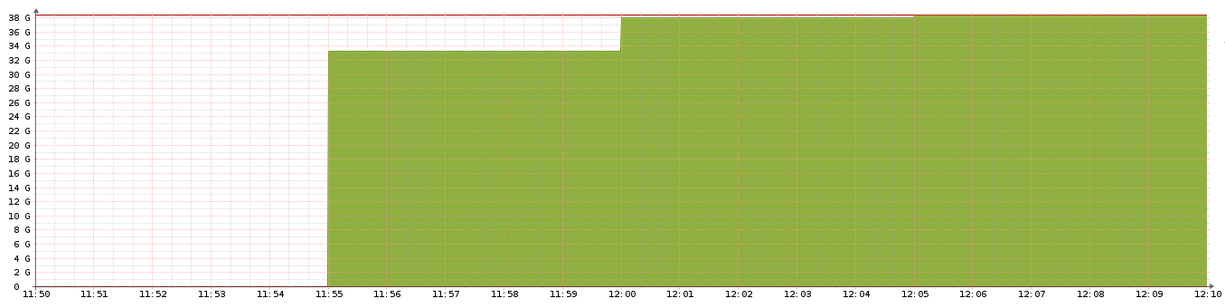
\includegraphics[scale=0.35]{images/pktgen_link_usage.png}
  \caption{Pktgen link usage for 400 byte packets (generated bandwidth at time x, graph displays an average of used bandwidth over 5 minutes}
  \label{fig:pktgenlink}
\end{figure}

\begin{figure}
  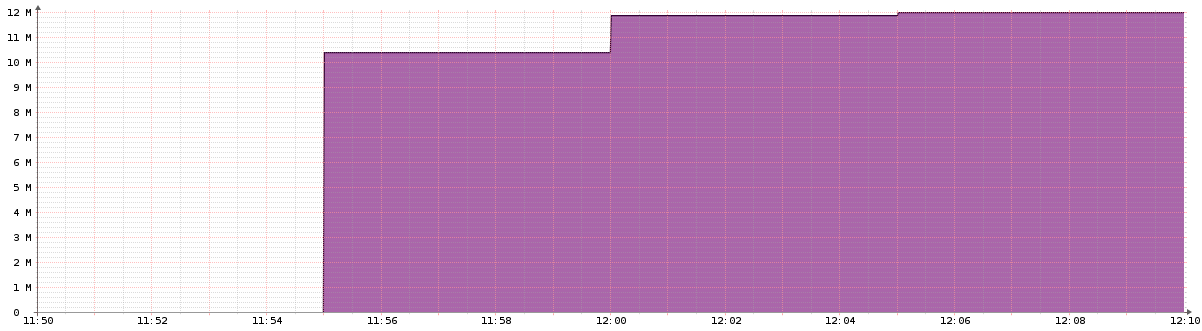
\includegraphics[scale=0.35]{images/pktgen_pps.png}
  \caption{Pktgen packets per second for 400 byte packets (generated packets per second at time x, graph displays the average transported pps over 5 minutes}
  \label{fig:pktgenpps}
\end{figure}

\newpage

\subsection{WARP}\label{sub:warp}
A WARP client needs a server to respond to SYN packets, otherwise sessions are not opened up and there will be no traffic flowing. 
WARP has to be tested against a WARP server or against an application server. 
Thus in a setup as the one used for the other tests, servers A and B both needed to run WARP, one as a server and one as a client generating requests. RAW TCP communication is chosen for a first test. 
Sending a request with the smallest possible Ethernet frame size of 64 bytes and responding with 64 bytes did not generate the maximum amount of pps expected, setting up the session using a three way handshake and transferring the data takes more CPU cycles, WARP seems to be limited regarding to the amount of packets per second it can send. WARP is capable of testing throughput up to the application level which makes it interesting for application layer testing.
To execute a benchmark for WARP, server B was connected to the network using two 40Gb/s interfaces back to back (both interfaces connected to the same card). One card is used for the server side of the benchmark, the other card is used for the client side of the benchmark. 
Since this test is focusing on the limitations of the server hardware the restrictions from RFC 2544 do not apply to this benchmark. Hence, tests do not have to run for 60 seconds.  
The benchmark increases the request and response sizes for every test. 4 million sessions are generated per test. The time it took to open and accept the sessions, transfer the data and then close all the opened sessions was registered. Tests were ran 3 times and the average value was written to a csv file. 
The results of this test for raw TCP traffic is shown in figures \ref{fig:rawtcplink} and \ref{fig:rawtcpsession}. 
WARP is also capable of testing HTTP session setup. The results of the benchmark for HTTP is visible in figures \ref{fig:httplink} and \ref{fig:httpsession}.
These figures show the packet sizes from the request and response along with the amount of sessions or the link usage.

WARP seems capable of generating 1 million session per second from the client side for raw TCP and HTTP traffic. The values shown display a requested amount of almost 1 million session per second. The server part of the application is not capable of responding to all the opened sessions when packet sized increase. The server gets overloaded by the client. The responses handled by the server side generate a total bandwidth of almost 50\% of the links bandwidth.  

\begin{figure}[H]
  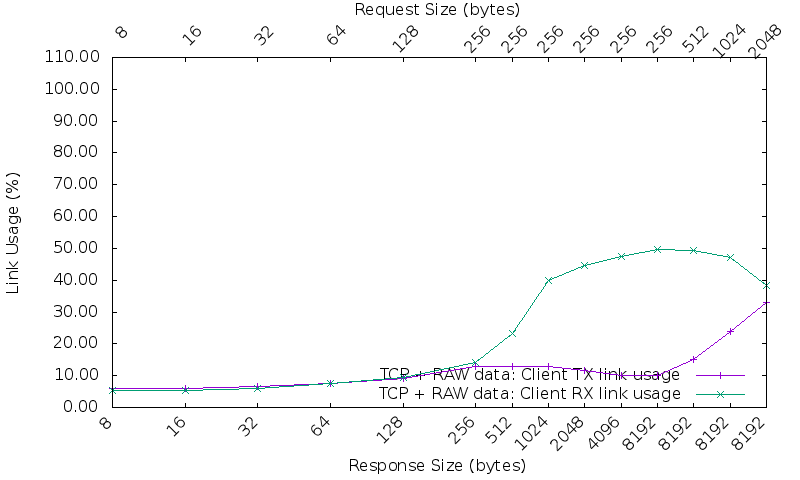
\includegraphics[scale=0.6]{images/raw_link_usage.png}
  \caption{Link usage for raw TCP (percentage of link usage versus the request(Rx) and response(Tx) size)}
  \label{fig:rawtcplink}
\end{figure}

\begin{figure}[H]
  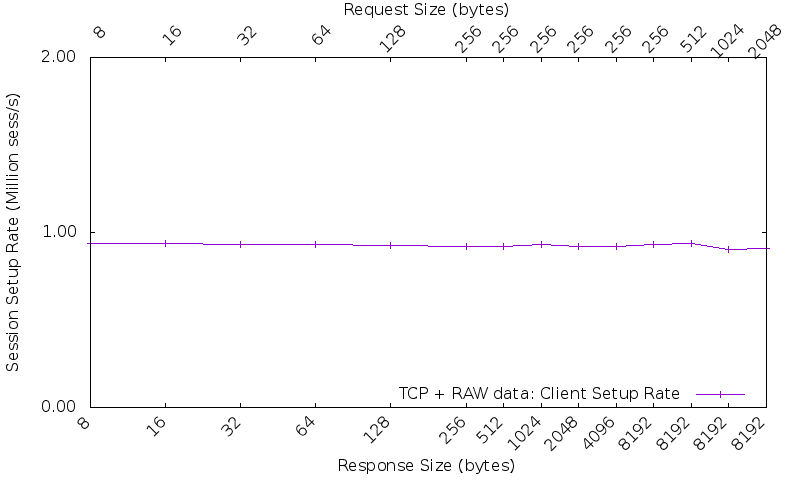
\includegraphics[scale=0.6]{images/raw_setup.png}
  \caption{Amount of requested session per second from the client to the server for raw TCP (amount of requested sessions versus the request(Rx) and respond(Tx) size)}
  \label{fig:rawtcpsession}
\end{figure}

\begin{figure}[H]
  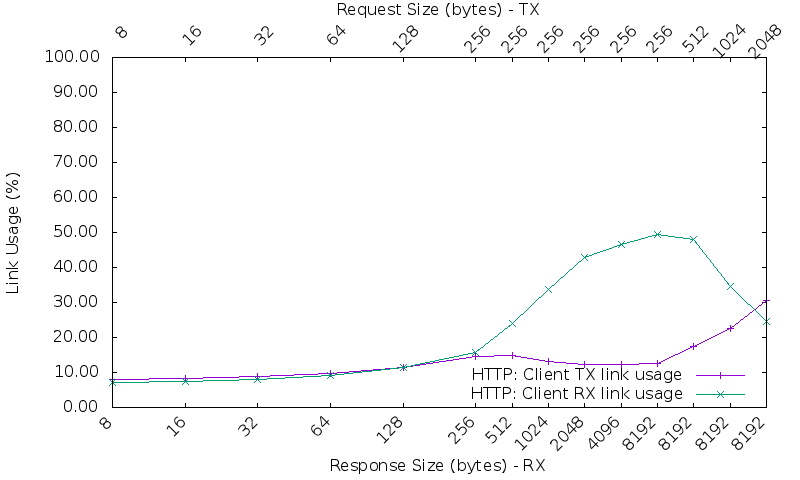
\includegraphics[scale=0.6]{images/http_link_usage.png}
  \caption{link usage for HTTP  (percentage of link usage versus the request(Rx) and response(Tx) size)}
  \label{fig:httplink}
\end{figure}

\begin{figure}[H]
  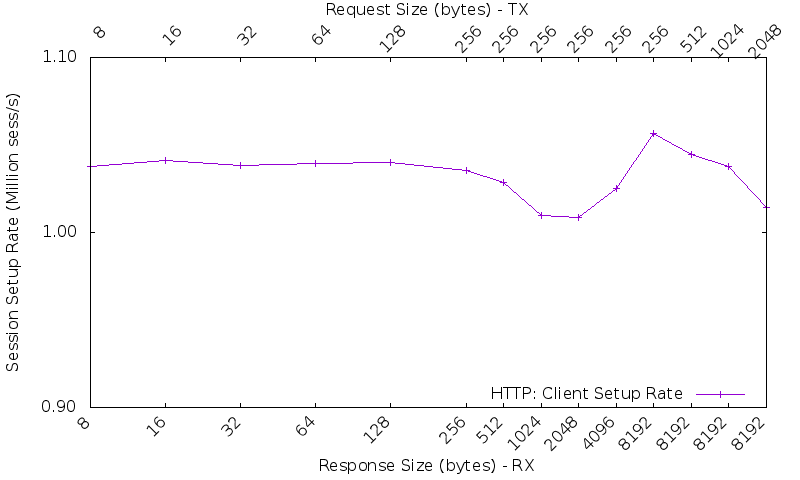
\includegraphics[scale=0.6]{images/http_setup.png}
  \caption{Amount of requested sessions per second from the client to the server for HTTP (amount of requested sessions versus the request(Rx) and respond(Tx) size)}
  \label{fig:httpsession}
\end{figure}


\subsection{MoonGen}
MoonGen offers benchmark scripts to determine the machines capabilities. A single machine (B) is connected to the switch using two 40Gb/s NIC's back to back (one NIC for the server part and the other for the clients part of the benchmark). Sending UDP traffic with a size of 1500 bytes resulted in a maximum of 24 Gb/s. When the smallest possible Ethernet packets of 64 bytes are send over the line a maximum of 15Mpps is reached. When TCP is used on the same machine (B) connected to the switch using two interfaces, a maximum of 10Gb/s was reached. These low values did not make MoonGen interesting enough since Pktgen is capable of reaching hardware limits. 


